\documentclass{beamer}
\usetheme{Boadilla}
\usepackage{graphicx}
\usepackage{listings}
\usepackage{color}
\graphicspath{ {./images/} }
\usepackage{float}
\usepackage[caption = false]{subfig}
\begin{document}

\title{Mandatory 3}
\subtitle{IN5450}
\author{Espen Lønes}
\institute{}
\date{\today}

\begin{frame}
	\titlepage
\end{frame}

\begin{frame}
	\frametitle{}
    \begin{itemize}
    \item Pulse compression
    \item Virtual array
    \item DAS
    \item TDMA / CDMA 
    \item Hamming tapering
    \item Using virtual array positions
    \end{itemize}
\end{frame}

\begin{frame}
	\frametitle{Overview}
	\begin{itemize}
		\item LFM pulse
		\item Pulse length 10 ms
		\item Bandwidth 10 kHz
		\item Center frequency 10 kHz
		\item 2 transmitters
		\item 32 receivers
		\item c = 340 m/s 
		\item TDMA data [Nt, Nrx, Ntx]
		\item Upchirp for both transmits
		\item CDMA data [Nt, Nrx]
		\item Down for left transmit, Up for right.
	\end{itemize}
\end{frame}

\begin{frame}
	\frametitle{Pulse compression code}
	\begin{figure}
    	\subfloat{\includegraphics[scale=0.7]{compression_code.png}}
	\end{figure}

\end{frame}

\begin{frame}
	\frametitle{Pulse compression images}
	We see one reflector.
	\begin{figure}
    	\subfloat{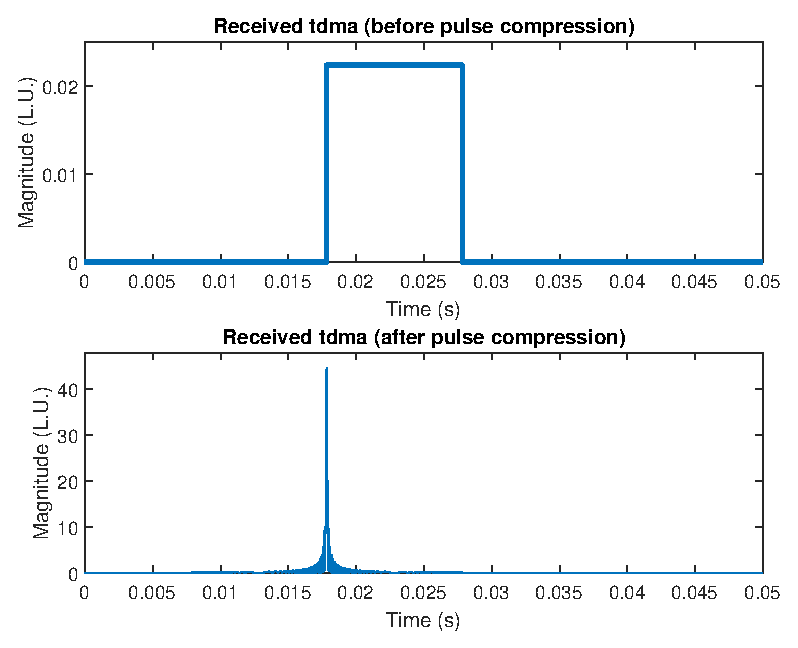
\includegraphics[scale=0.45]{compression_tdma.eps}}
    	\subfloat{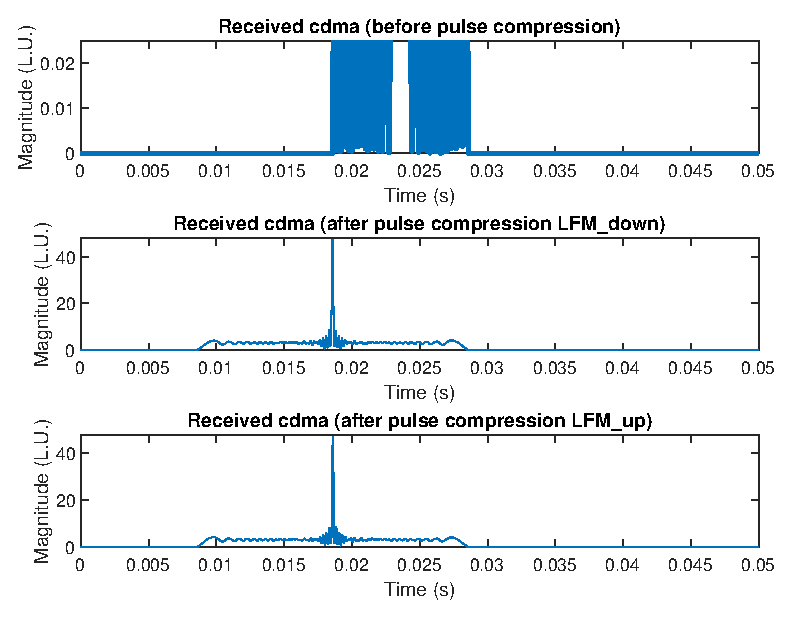
\includegraphics[scale=0.45]{compression_cdma.eps}}
	\end{figure}
    Theoretical time resolution = 1 / B = 1.0000e-04 = 0.0001 s.\\
    Measured resolution = 0.01792 - 0.017725 = 1.9500e-04 = 0.000195 s.\\
	Measured $\approx$ 2 * Theoretical\\
\end{frame}

\begin{frame}
	\frametitle{Virtual array}
	For one transmit sampling is half compared to using two transmits.\\
	(Array is also slightly longer for two transmits.)
	\begin{figure}
    	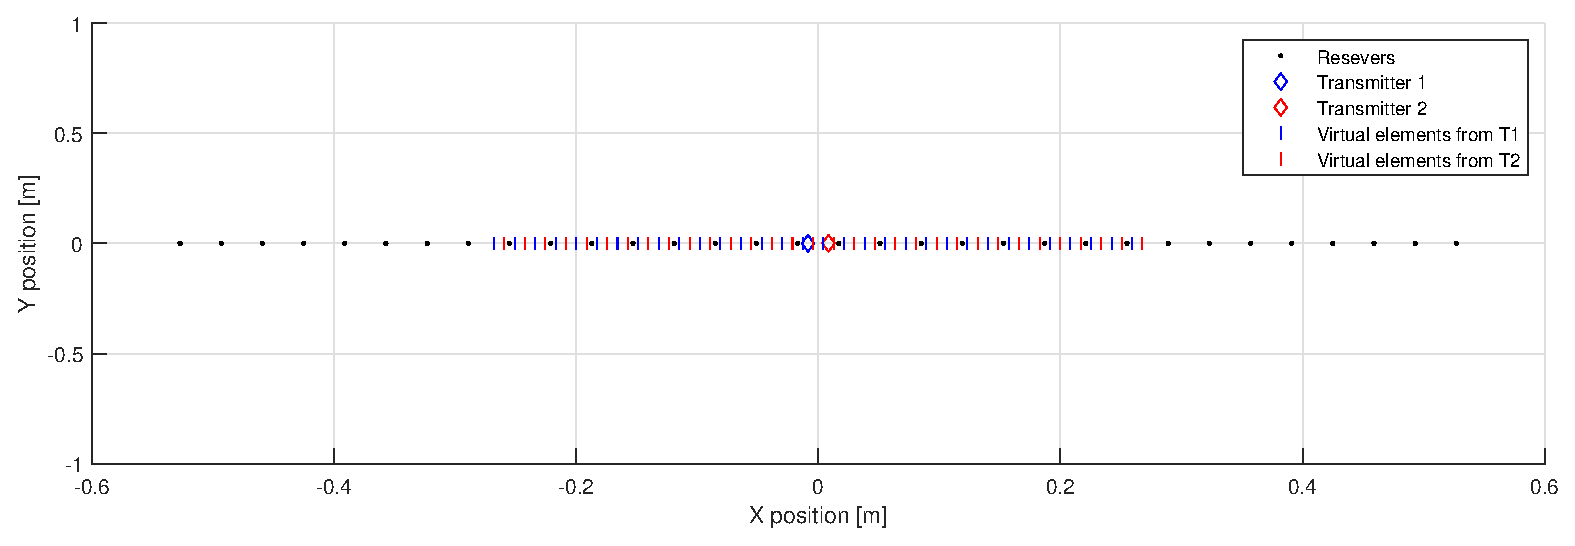
\includegraphics[scale=0.4]{Arrays.eps}\\	
	\end{figure}
    Theoretical lateral resolution $= \lambda / L = (c/fc) / (2*0.26775) = \frac{0.0340 }{0.		5355}$\\
    $= 0.0635[rad] = 3.638282[deg]$\\
    Approx lateral resolution at 4 m: $R*a = 4 * 0.0635 = 0.254 m$\\
    Theoretical axial resolution $= c / (2*B) = 0.0170 m$\\
    At 4 meters $0.254 / 0.0170 = 14.9$, axial is 15 times better than lateral.
\end{frame}

\begin{frame}[fragile]
	\frametitle{DAS code}
	\begin{figure}
		\includegraphics[scale=0.56]{das_code.png}\\
	\end{figure}
\end{frame}

\begin{frame}
	\frametitle{TDMA two transmits}
	Reflector is at [x,y] = [-1.3975, 2.8025] or [r, $\theta$] = [3.1316, 116.5037]\\
	Single point reflector. Axial pollution spans 2 * width of pulse.\\
	Theoretical lateral res.: $\frac{(c/fc)}{2 * 0.527} = 0.0323 [rad]$. 0.1012[m] at point.\\ 			Measured: $0.0951[m]$\\ 
	Theoretical axial res.: $c / (2*B) = 0.0170[m]$. Measured: $0.0140[m]$\\
	\begin{figure}
    	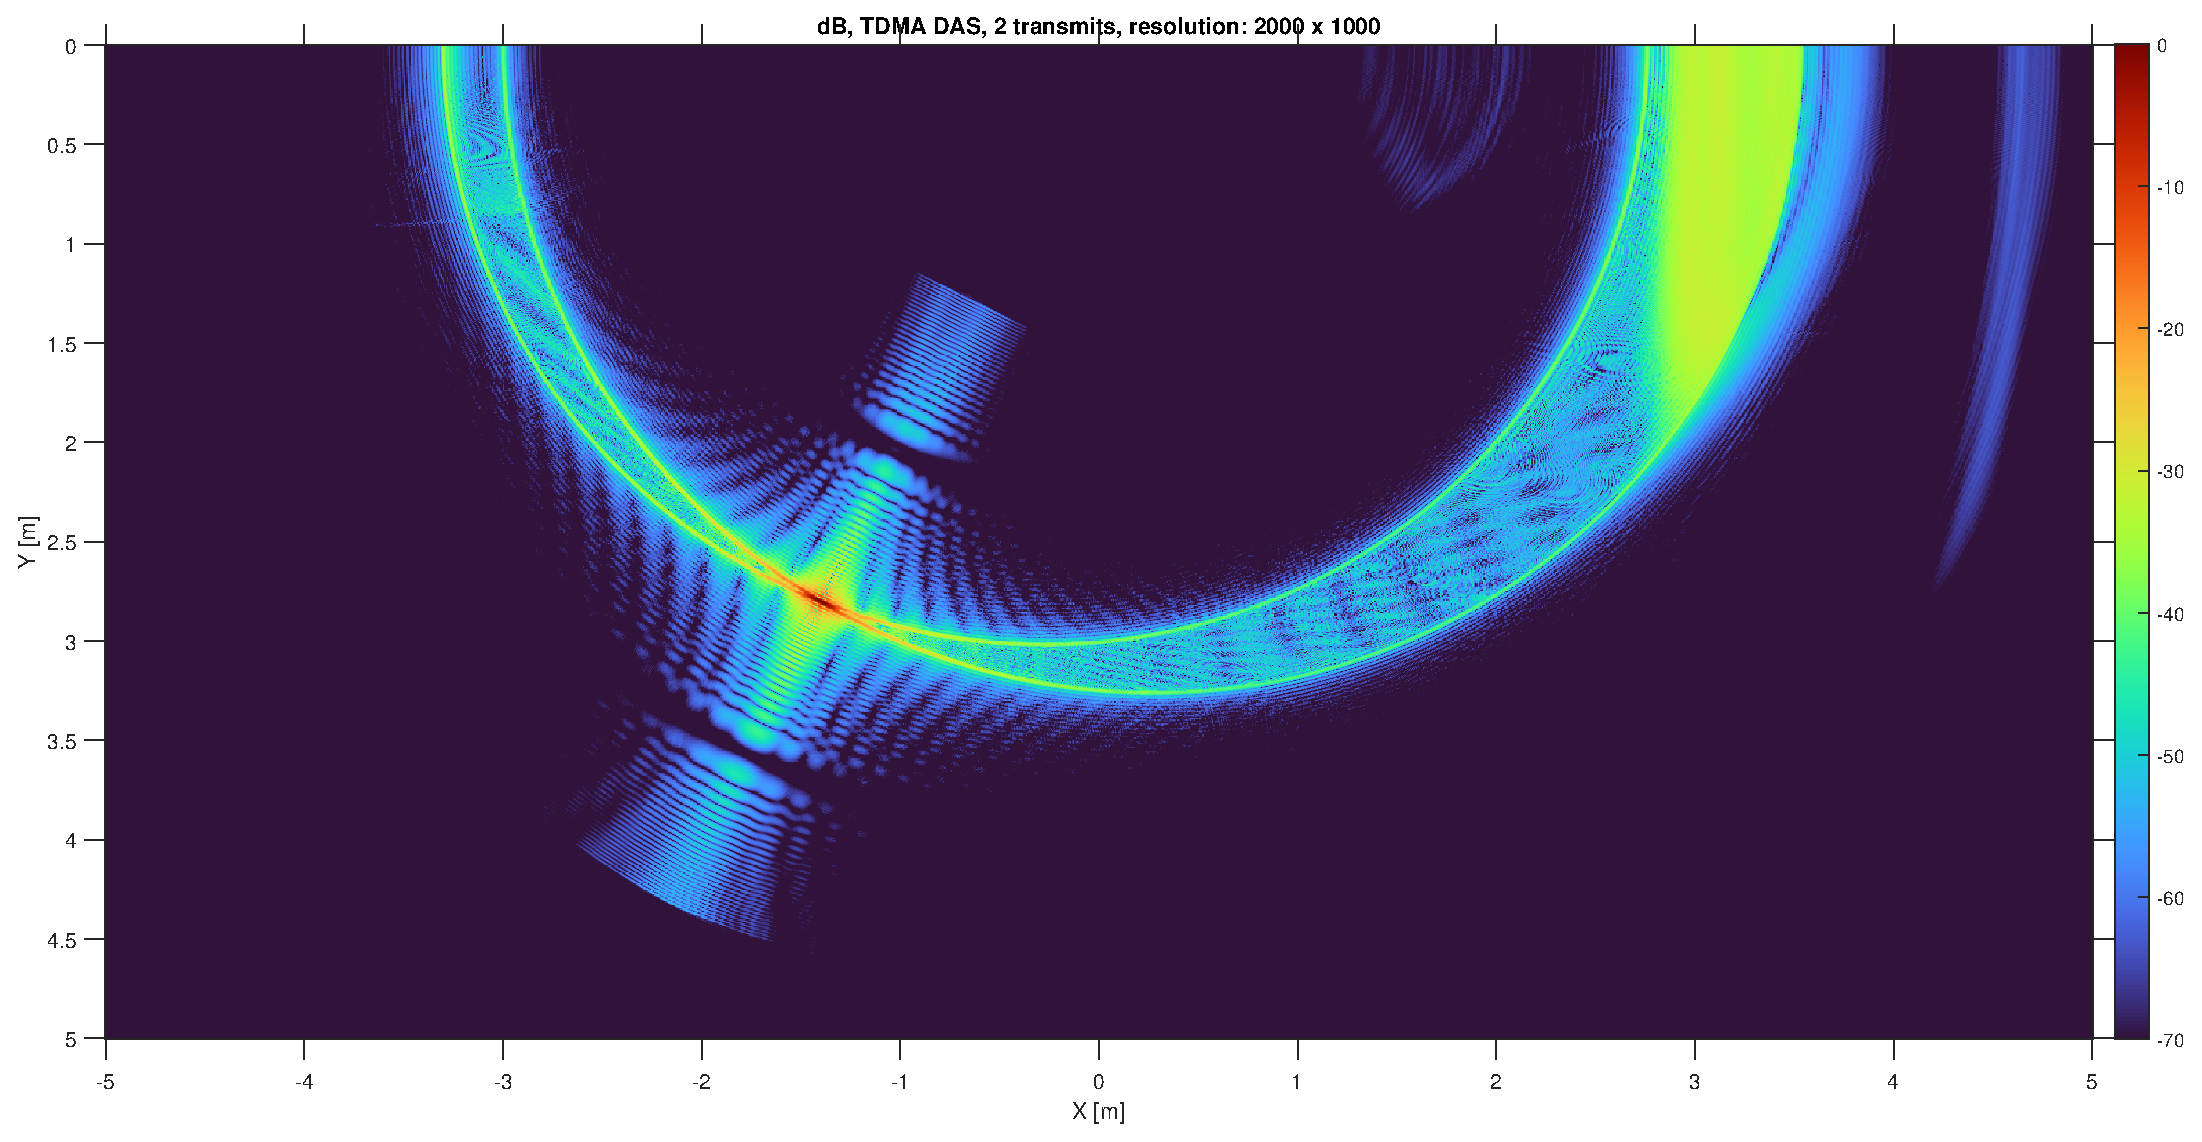
\includegraphics[scale=0.31]{tdma_2t.eps}\\	
	\end{figure}	
\end{frame}

\begin{frame}
	\frametitle{TDMA one transmit}
	Similar image around point but stronger/larger artefacts to the sides.\\
	\begin{figure}
    	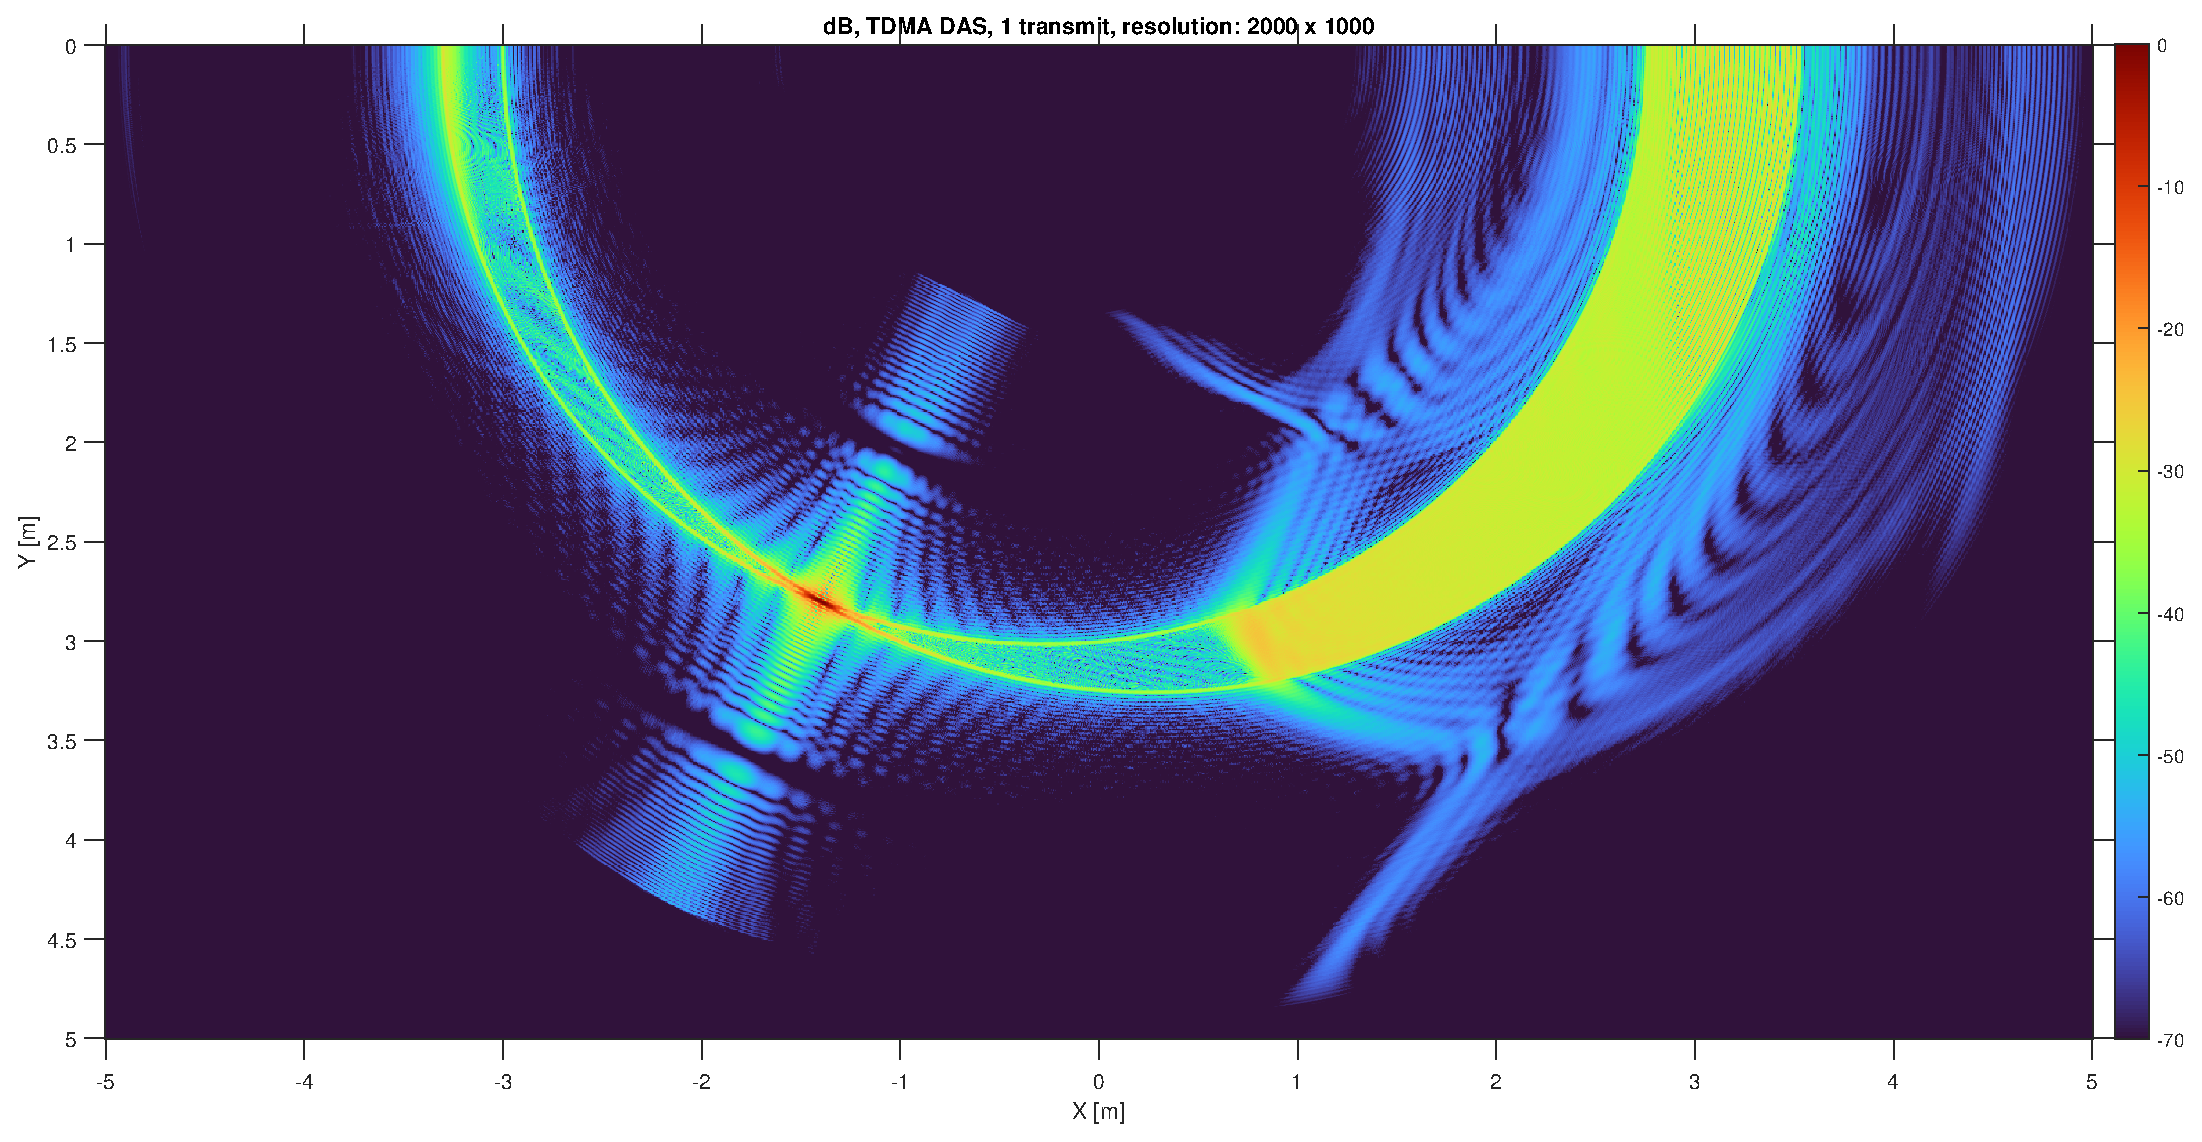
\includegraphics[scale=0.33]{tdma_1t.eps}\\	
	\end{figure}
\end{frame}

\begin{frame}
	\frametitle{CDMA plot}
	All over higher level of pollution than TDMA.\\
	(Higher 'baseline' pollution artefacts).\\
	Because the two pulses interfere slightly (provides nose for each other).\\
	Worse quality but half the imaging time.\\
	\begin{figure}
    	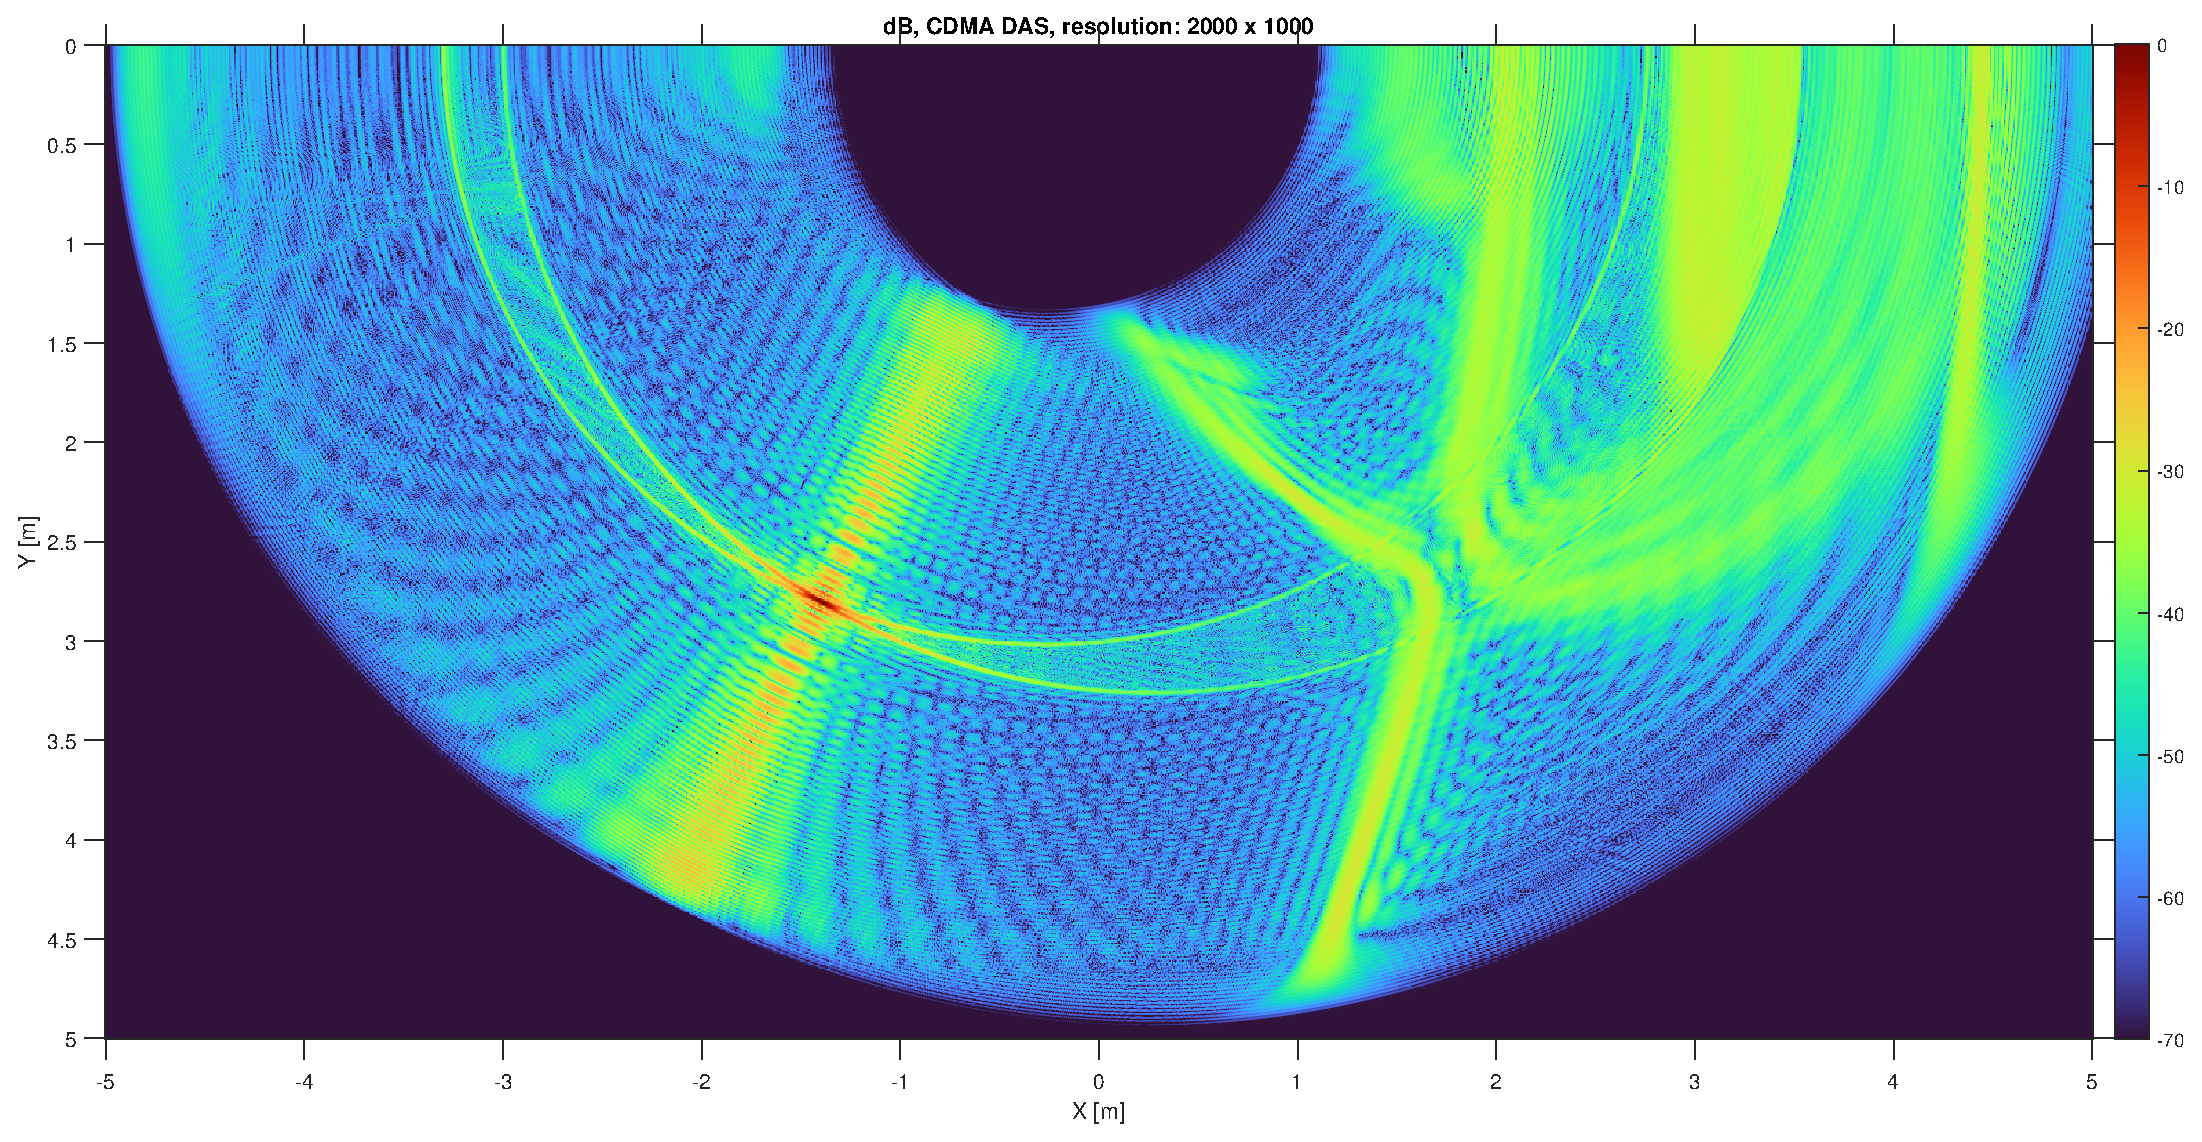
\includegraphics[scale=0.32]{cdma.eps}\\	
	\end{figure}
\end{frame}

\begin{frame}
	\frametitle{Hamming tapered full TDMA}
	Hamming tapering was used on receive array and transmit waveform.\\  	
	Less / smother artefacts, especially far to the sides.\\ 
	Worse resolution.\\
	\begin{figure}
    	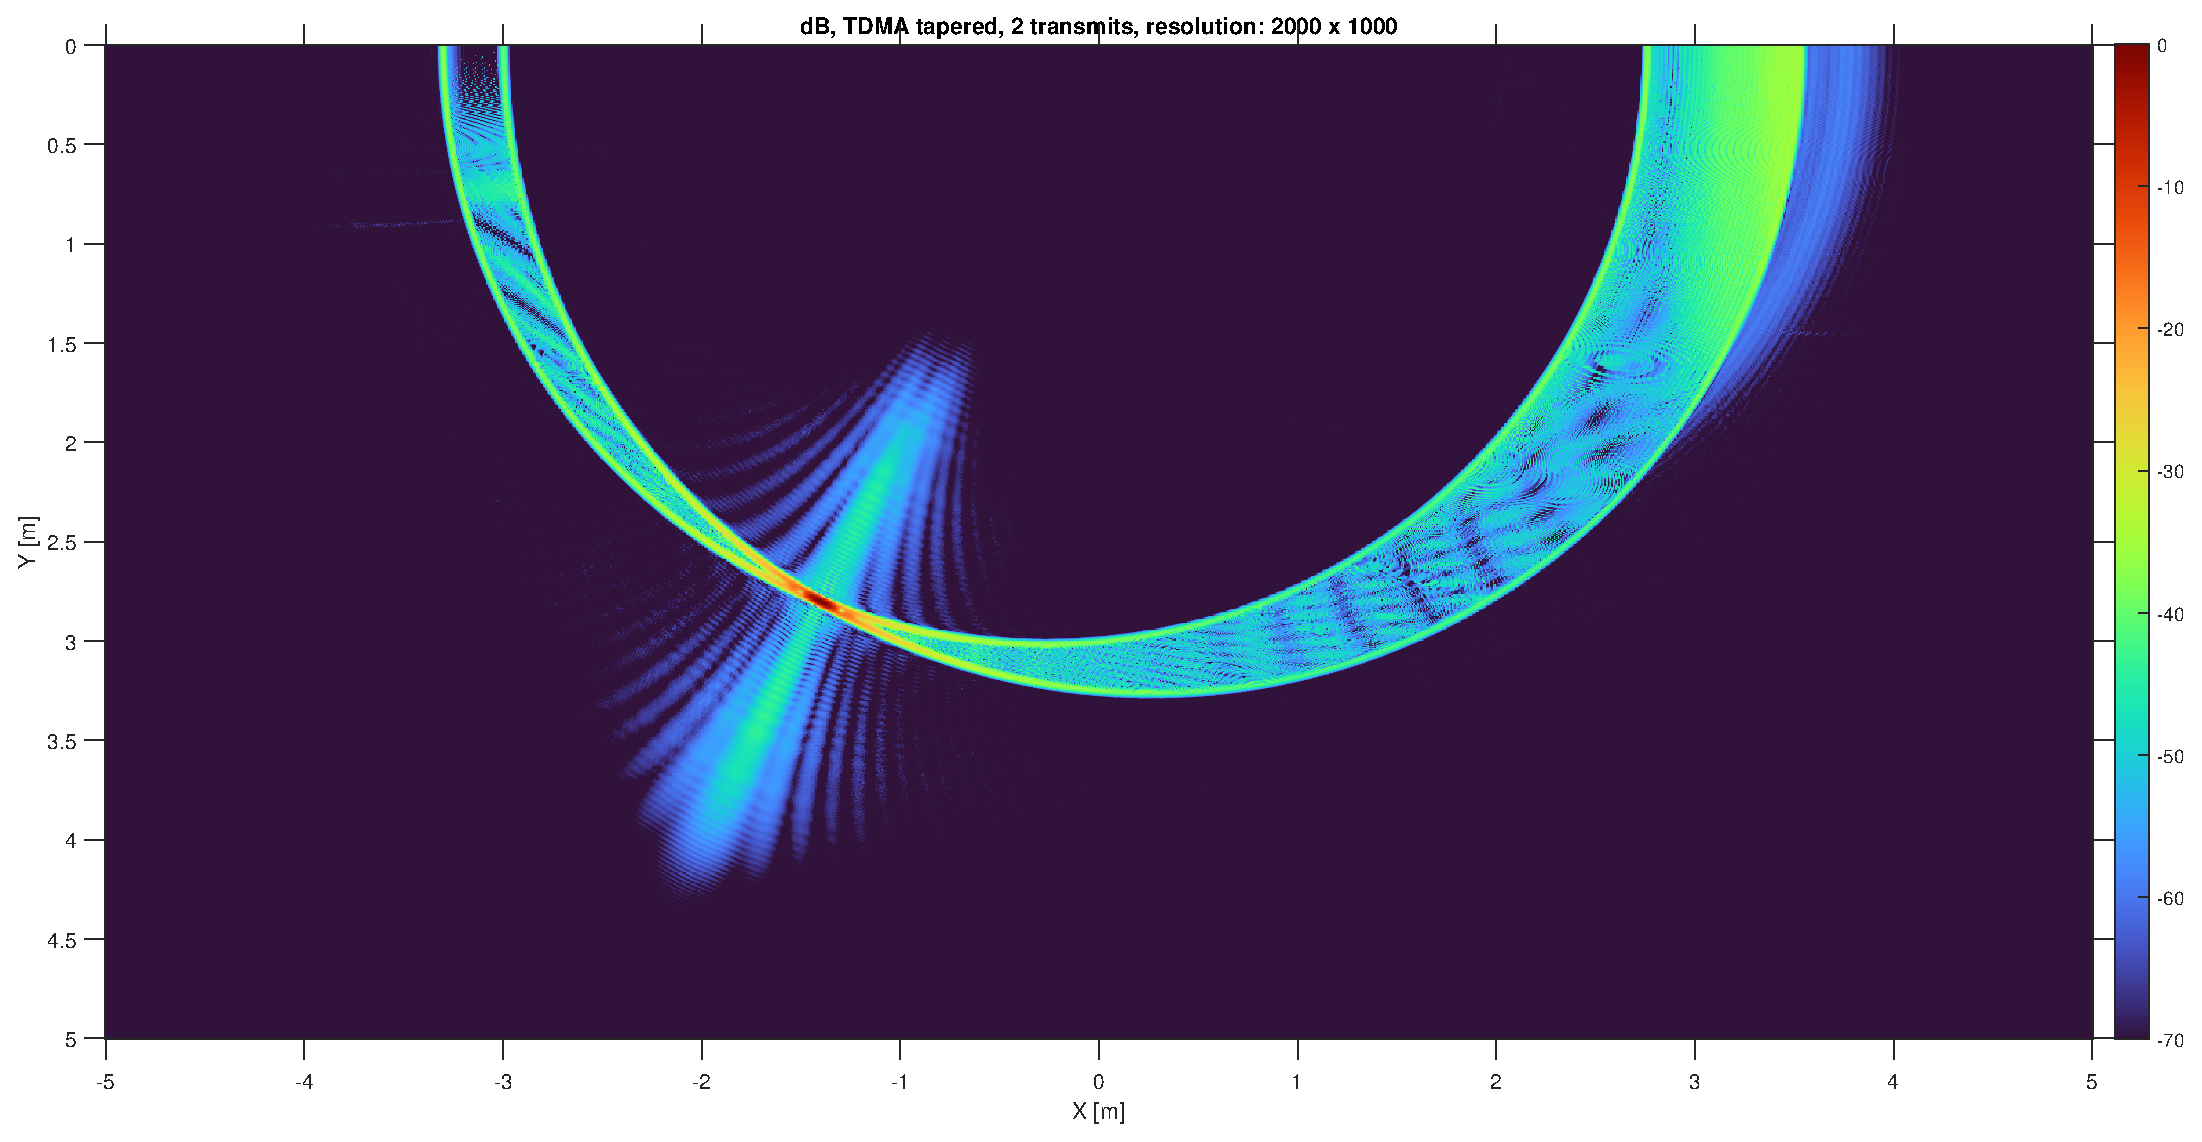
\includegraphics[scale=0.33]{tdma_2t_tapered.eps}\\	
	\end{figure}
\end{frame}

\begin{frame}
	\frametitle{Hamming tapered single transmit TDMA}
	Hamming tapering was used on receive array and transmit waveform.\\  	
	Again worse resolution.\\
	Partially removes and smooths some of the single transmit artefacts.\\ 
	\begin{figure}
    	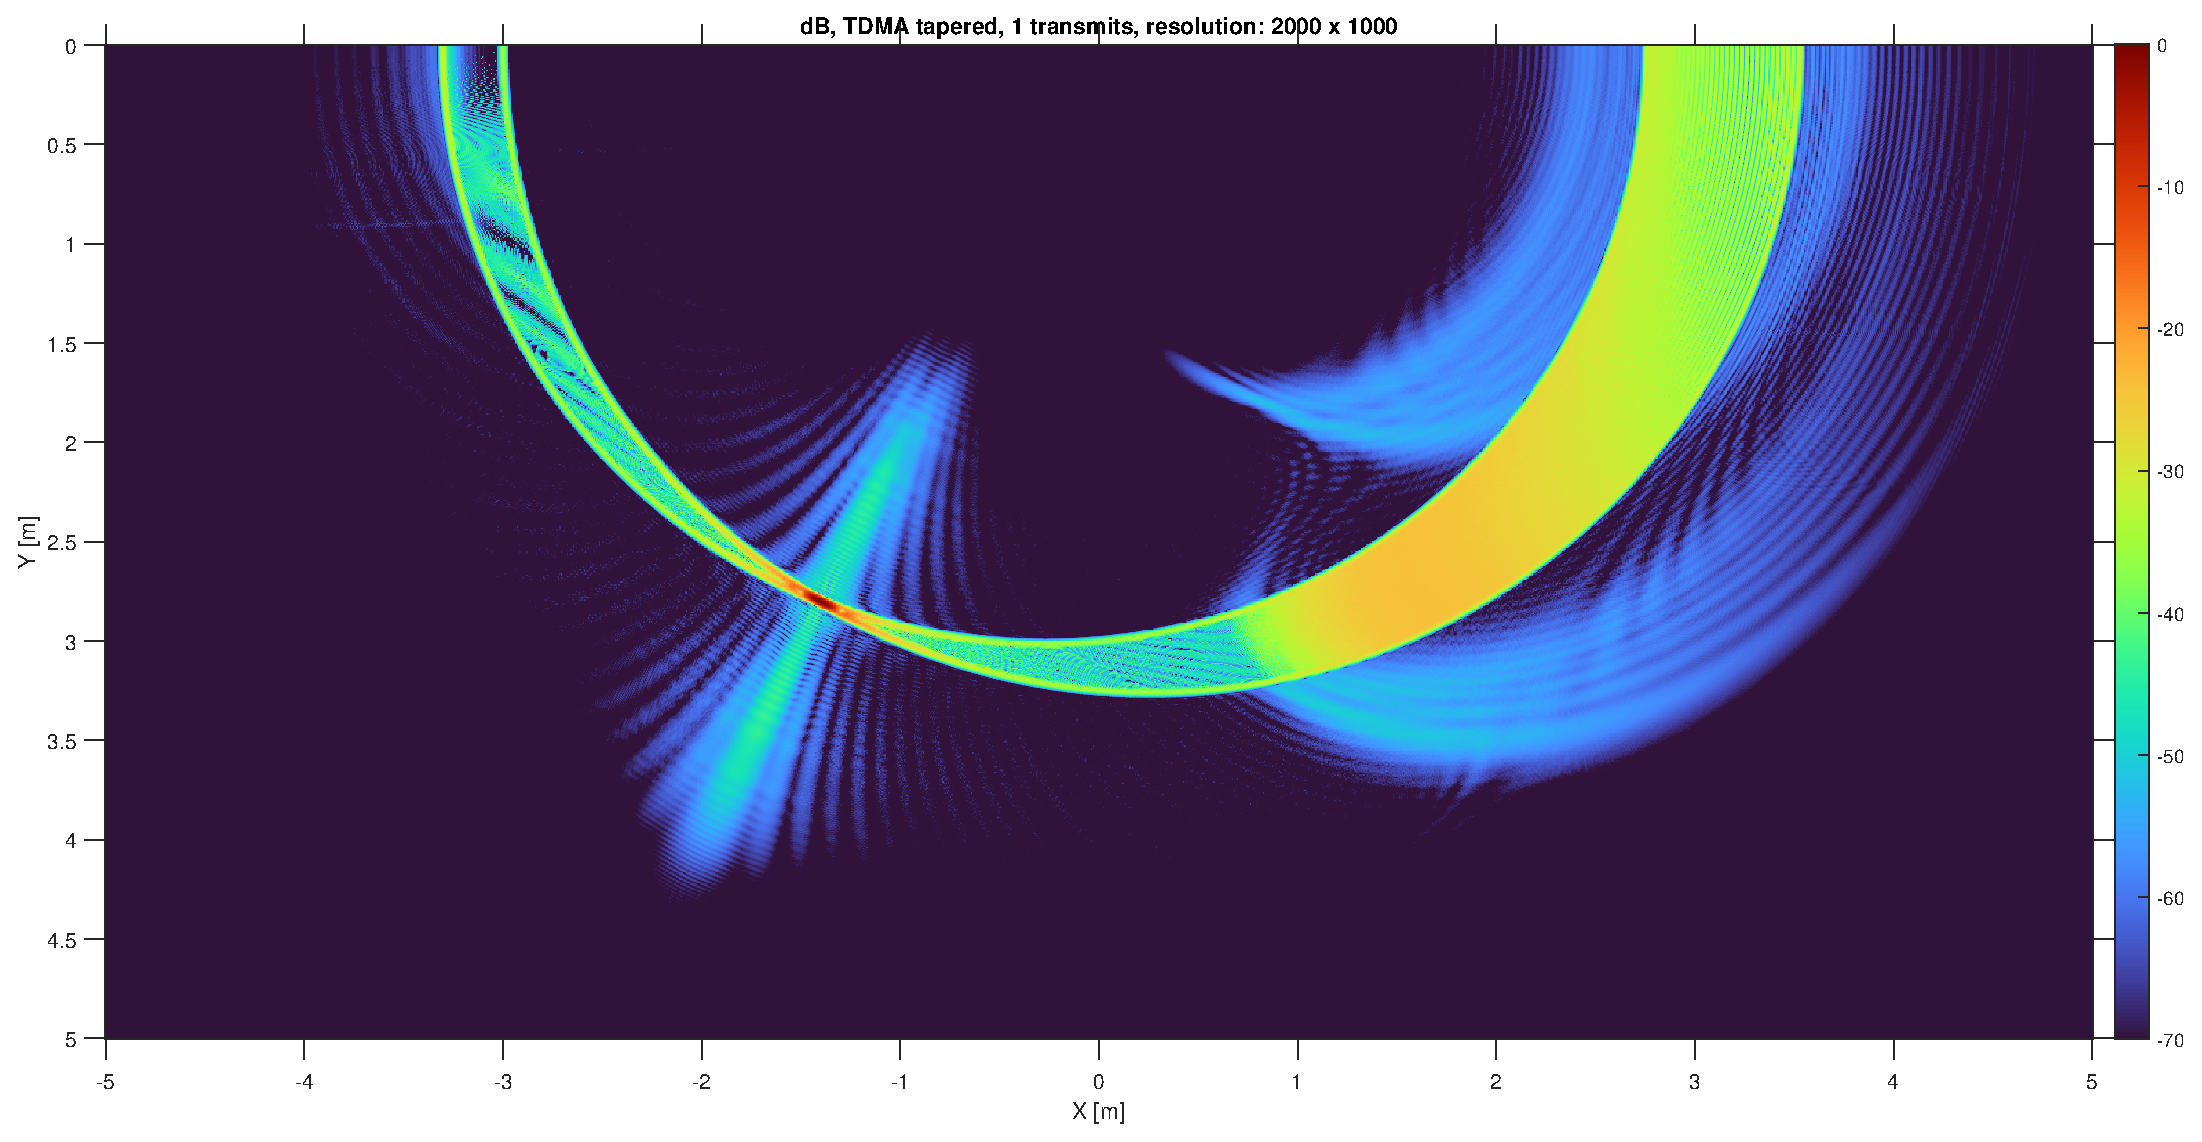
\includegraphics[scale=0.32]{tdma_1t_tapered.eps}\\	
	\end{figure}
\end{frame}

\begin{frame}
	\frametitle{TDMA with virtual array positions} 	
	Equal axial resolution. ($\frac{1}{B}$)\\ 
	Worse lateral resolution because of shorter array length. ($\frac{\lambda}{L}$).\\ 
	0.0323[rad] vs. 0.0635[rad]\\
	\begin{figure}
    	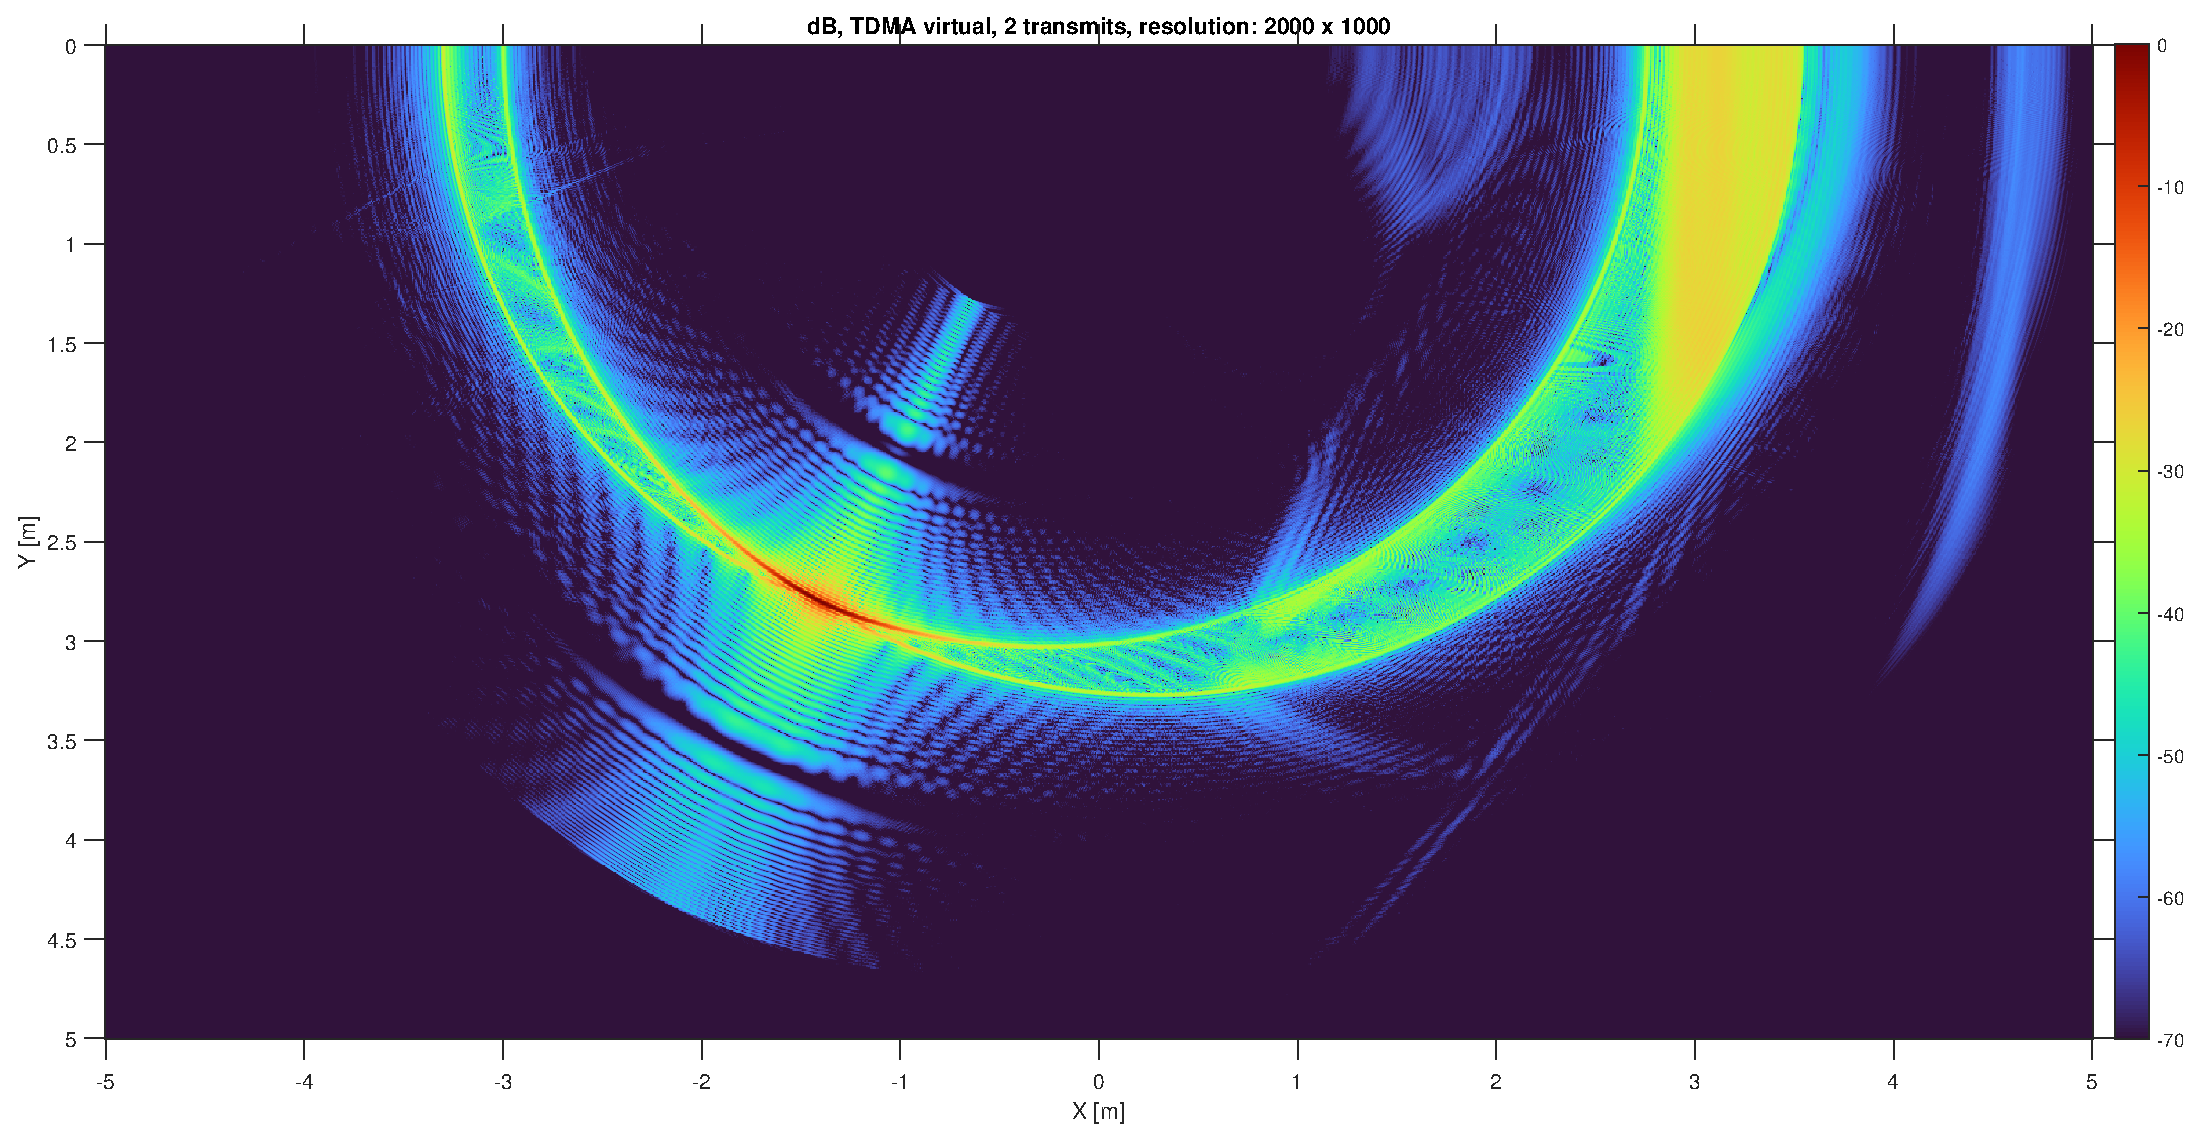
\includegraphics[scale=0.33]{tdma_2t_virtual.eps}\\	
	\end{figure}
\end{frame}

\begin{frame}
	\frametitle{References}
	\begin{itemize}
		\item \url{https://www-int.uio.no/studier/emner/matnat/ifi/IN5450/v22/undervisningsmateriale/mandatory_three/in5450_mimo_project_2022.pdf}	
	
		\item \url{https://www-int.uio.no/studier/emner/matnat/ifi/IN5450/v22/undervisningsmateriale/in5450\_mimo\_2022\_v1\_handout\_compressed.pdf}
		
		\item \url{https://www-int.uio.no/studier/emner/matnat/ifi/IN5450/v22/undervisningsmateriale/in5450\_saft\_2022\_v1\_handout\_compressed.pdf}
		
		\item \url{https://www-int.uio.no/studier/emner/matnat/ifi/IN5450/v22/undervisningsmateriale/in5450\_sas\_2022\_v1\_handout\_compressed.pdf}
	\end{itemize}
\end{frame}

\end{document}